%%%%%%%%%%%%%%%%%%%%%%%%%%%%%%%%%%%%%%%%%%%%%%%%%%%%%%%%%%%%%%%%%
% Tese de Doutorado / Dept Fisica, CFM, UFSC                    %
% Andre@UFSC - 2014                                             %
%%%%%%%%%%%%%%%%%%%%%%%%%%%%%%%%%%%%%%%%%%%%%%%%%%%%%%%%%%%%%%%%%

%:::::::::::::::::::::::::::::::::::::::::::::::::::::::::::::::%
%                                                               %
%                          Capítulo 7                           %
%                                                               %
%:::::::::::::::::::::::::::::::::::::::::::::::::::::::::::::::%

%***************************************************************%
%                                                               %
%                        Decomposicao                           %
%                                                               %
%***************************************************************%

\chapter{Decomposição morfológica espectral de galáxias}
\label{sec:Decomp}

%***************************************************************%
%                                                               %
%               Decomposição: decomposicao espectral            %
%                                                               %
%***************************************************************%

\section{O procedimento de decomposição morfológica espectral}

A decomposição morfológica espectral apresentada neste capítulo foi desenhada
para trabalhar com galáxias lenticulares (S0), que podem ser decompostas em um
bojo e um disco. Conforme a Seção \ref{sec:morph:comp:bd}, o perfil de brilho do
bojo é modelado como uma lei de Sérsic, e o perfil do disco como uma lei
exponencial, conforme as equações
\begin{equation*}
I(r) = I_e \exp \left\{- b_n \left[ \left( \frac{r}{r_e} \right)^{1/n}
- 1 \right] \right\},
\end{equation*}
\begin{equation*}
I(r) = I_0 \exp\left(- \frac{r}{h}\right).
\end{equation*}

Diferente do método de \citeauthor{Johnston2012}, os perfis do bojo e do disco
são tratados em duas dimensões como elipsoides, cada qual com uma elipticidade
($\epsilon$) e um ângulo de posição (P.A.) independentes. O ângulo de posição é
medido em sentido anti-horário a partir do eixo horizontal positivo. Estes
modelos são ajustados a imagens em cada comprimento de onda, utilizando o
programa IMFIT, conforme descrito na seção a seguir. A decomposição é realizada
sobre os espectros observados. As linhas de emissão são mascaradas, pois estamos
interessados apenas na distribuição de populações estelares.
O ajuste morfológico é feito deixando livres todos os parâmetros das equações
acima ($I_e$, $r_e$, $n$, $I_0$, $h$) e a geometria de cada componente (P.A. e
$\epsilon$), sem fazer hipótese alguma sobre como os parâmetros morfológicos
variam a cada comprimento de onda.

Conforme descrito na Seção \ref{sec:psf:medida}, convoluem-se as imagens do
modelo com uma PSF de perfil de Moffat com $\beta=4$ e
$\mathrm{FWHM}=2,9\,\arcs$. Possíveis efeitos causados por uma PSF mal
dimensionada foram vistos na Seção \ref{sec:test:psf}. Esta é uma preocupação
muito relevante no caso do CALIFA, pois em geral os bojos estão mal resolvidos.

% TODO: repensar esta seção sobre python-imfit.
%\subsection{A biblioteca python-imfit}

%\TODO vender o jabá - mini-tutorial do python-imfit?


\subsection{Cinemática}
\label{sec:Decomp:cinematica}

Antes de começar a decomposição, é preciso refletir um pouco sobre a cinemática
das estrelas da galáxia. As estrelas estão distribuídas em bojos e discos, e a
cinemática em cada um dos casos é diferente.
A estrutura plana dos discos é causada por um alto momento angular, com um campo
de velocidades sistêmico projetado na linha de visada. Isto faz com que uma dada
linha espectral tenha um {\em redshift} diferente, dependendo da sua posição no
disco. Já os bojos são normalmente caracterizados por baixa rotação, mas uma
grande dispersão de velocidades, crescendo à medida que se aproxima do centro.
Ou seja, as linhas são mais alargadas nas regiões centrais.

Para que a decomposição morfológica espectral faça sentido, é preciso ter
certeza que, em uma imagem em uma dada janela espectral, se estejam observando
os mesmos processos físicos em todos os {\em spaxels}. Por exemplo, não se pode
ter um {\em spaxel} que contenha fluxo proveniente do fundo de uma linha de
absorção, enquanto outro {\em spaxel} contém fluxo do contínuo adjacente.
Chega-se então num problema cíclico. É preciso saber as características das
componentes morfológicas para que se conheça a cinemática de cada uma delas.
Porém, sem compensar os efeitos da cinemática, não se pode fazer a decomposição
de forma confiável.

O que se faz aqui é obter uma medida aproximada da cinemática, medindo apenas
uma velocidade sistêmica ($v_0$) e uma dispersão ($v_d$) assumindo uma
distribuição de velocidades gaussiana para cada {\em spaxel}. Isto não é o
ideal, pois bojos podem ter alguma rotação e discos podem ter alguma dispersão
de velocidades. A cinemática pode até ser diferente para cada cada população
estelar em uma mesma componente. Entretanto, isto é uma boa primeira
aproximação. A medida de $v_0$ e $v_d$ foi obtida utilizando o \starlight, que
ajusta a cinemática juntamente às populações estelares.

Corrigir efeitos de $v_0$ é simples, basta aplicar um {\em redshift} (ou {\em
blueshift}) de mesma velocidade, na direção oposta, tal que os espectros fiquem
todos em {\em rest frame}. Já $v_d$ requer um pouco mais de consideração, pois
não é possível ``desalargar'' as linhas espectrais. O que se faz então é tentar
deixar todos os {\em spaxels} com a mesma dispersão de velocidades, degradando a
resolução do espectro. Se a distribuição de velocidades na linha de visada segue
uma distribuição gaussiana, isto é obtido convoluindo (em espaço de velocidades)
o fluxo cada {\em spaxel} com uma gaussiana de largura dada por um $v_{d,\ast}$
adequado, isto é
\begin{equation*}
F_{\lambda,\ast} = \frac{1}{v_{d,\ast}\sqrt{2\pi}}\int_{-\infty}^{+\infty}
F_\lambda \left(\lambda^\prime = \frac{\lambda}{1 + v/c}\right) \exp \left[ -\frac{1}{2}
(v/v_{d,\ast})^2 \right] \mathrm{d}v.
\end{equation*}
Quando se convolui duas gaussianas, suas dispersões se somam em
quadratura. Portanto, $v_{d,\ast}$ deve ser tal que o fluxo final tenha a
dispersão alvo $v_{d,\mathrm{alvo}}$:
\begin{equation*}
v_{d,\ast} = \sqrt{v_{d,\mathrm{alvo}} - v^2_d}.
\end{equation*}

\begin{figure}
	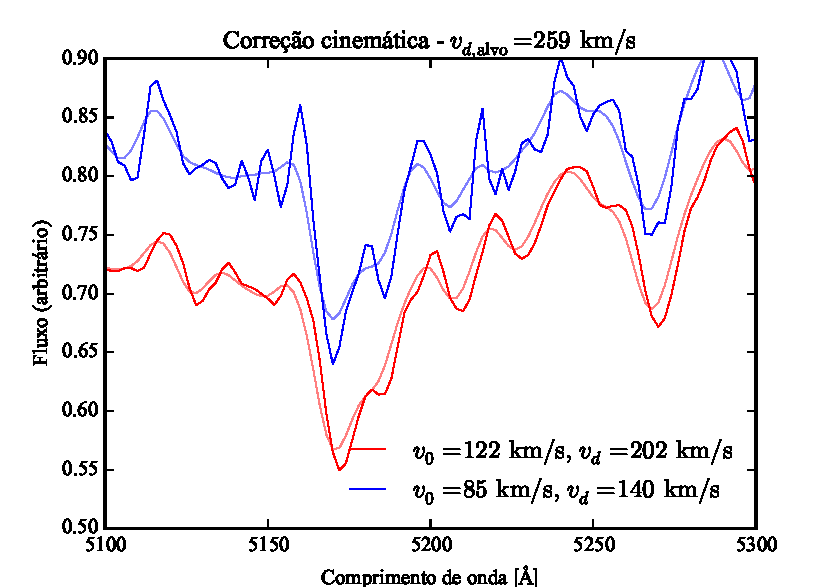
\includegraphics{figuras/cinematica}
	\caption[Correção de efeitos da cinemática]
	{Correção de efeitos da cinemática. Linhas escuras: dois espectros com
	cinemática diferente. Linhas claras: espectros deslocados para {\em rest
	frame}, com as linhas alargadas para uma dispersão de velocidades
	$v_{d,\mathrm{alvo}} = 259\,\mathrm{km}/\mathrm{s}$. O fluxo está em unidades
	arbitrárias para melhor visualização.}
	\label{fig:cinematica}
\end{figure}

Deve-se escolher $v_{d,\mathrm{alvo}}$ de modo que $v_{d,\ast}$ seja sempre um
número real, ou seja, $v_{d,\mathrm{alvo}} > v_d$, para todos os {\em spaxels}.
Na prática, alguns cubos podem ter uns poucos {\em spaxels} com $v_d$ anômalo
(tanto por ajuste ruim pelo \starlight quanto por uma dispersão realmente
grande). Neste caso, a resolução espectral seria degradada enormemente por conta
de um punhado de {\em spaxels}. A solução encontrada foi usar um
$v_{d,\mathrm{alvo}}$ maior do que $95\%$ dos $v_d$, e não fazendo a convolução
nos poucos casos onde $v_d > v_{d,\mathrm{alvo}}$. A Figura \ref{fig:cinematica}
ilustra o efeito da correção de cinemática em {\em spaxels} com cinemática
distinta. Pode-se ver que as linhas espectrais tendem a ficar coerentes após a
correção.


\subsection{Propagação de erros nos espectros}

Em alguns passos da decomposição, são tomadas imagens dos cubos espectrais em
caixas com uma determinada largura em comprimento de onda. Os espectros são
empilhados formando uma imagem, e os erros devem ser propagados de acordo. Os
espectros do CALIFA, na configuração V500, têm uma PSF espectral gaussiana de
$\mathrm{FWHM}=6\,\angstrom$. Porém, a amostragem é feita em caixas de
$2\,\angstrom$. Isto que dizer que fluxos estão correlacionados, logo deveria-se
trabalhar com a matriz de covariância, ao invés de um espectro de erros (ou
incerteza). Entretanto, somente o espectro de erros está disponível nos cubos de
dados do CALIFA (e na maioria dos espectros astronômicos). Note que o mesmo
raciocínio de propagação de erros se aplica à correção de cinemática descrita
anteriormente, com a gaussiana da dispersão de velocidades fazendo o papel de um
peso na soma dos espectros.

Sem a matriz de covariância, há duas alternativas. Se erros nos fluxos estão
correlacionados com dependência na distância espectral de forma a depender
apenas da distância, isto é, uma função $p(\lambda^\prime -
\lambda^{\prime\prime})$, pode-se calcular a correção que a covariância causaria
numa soma ponderada de fluxo. O fluxo médio $F$ ponderado pelos pesos
$w_\lambda$ é dado por
\begin{equation*}
F = \frac{\sum\limits_\lambda w_\lambda F_\lambda}{\sum\limits_\lambda
w_\lambda}.
\end{equation*}
Geralmente se normalizam os erros tal que $\sum\limits_\lambda
w_\lambda = 1$, para simplificar os cálculos. O erro $\sigma_F$ sobre o fluxo
médio $F$ é, levando em conta a correlação,
\begin{equation*}
\sigma_F^2 = \sum\limits_\lambda w_\lambda^2 \sigma_\lambda^2 +
\sum\limits_{\lambda^\prime}
\sum\limits_{\lambda^{\prime\prime}}^{\lambda^{\prime\prime} \neq
\lambda^\prime} p(\lambda^\prime - \lambda^{\prime\prime}) w_{\lambda^\prime}
w_{\lambda^{\prime\prime}} \sigma_{\lambda^\prime}
\sigma_{\lambda^{\prime\prime}}.
\end{equation*}
Para erros gaussianos, $p(\Delta \lambda) \sim \exp\left[-1/2
(\Delta\lambda / c_\mathrm{FWHM})^2\right]$, normalizado. A distância de
covariância é dada por $\mathrm{FWHM} = 2 \sqrt{2 \ln 2}\ c_\mathrm{FWHM}$. Se
os erros não estiverem correlacionados (isto é, se $\mathrm{FWHM} \to 0$),
$p(\Delta \lambda) = 0$, a segunda soma desaparece e o erro é dado pela soma
ponderada usual.

A segunda alternativa é estimar o erro a partir dos dados. Isto só funciona
quando a soma é feita sobre uma caixa espectral com um grande número de medidas.
Neste caso, o erro é dado pela covariância amostral,
\begin{equation*}
\sigma_F^2 = \dfrac{\sum\limits_\lambda w_\lambda}{\left(\sum\limits_\lambda
w_\lambda\right)^2 - \sum\limits_\lambda w_\lambda^2} \sum\limits_\lambda
w_\lambda \left(F_\lambda - F\right)^2.
\end{equation*}

A primeira alternativa é utilizada na convolução de velocidades, pois em geral
cada elemento do espectro convoluído contém fluxo proveniente de poucas medidas.
A segunda é utilizada ao se empilhar espectros em caixas de comprimento de onda
de largura maior que $100\,\angstrom$, para uma estimativa mais realista do
erro. Quando se calcula a imagem média numa caixa, neste trabalho, o peso na
soma ponderada dos fluxos é dado por $w_\lambda = \sigma_\lambda^{-2}$, ou seja,
o inverso dos erros provenientes dos cubos de dados, ao quadrado.


\subsection{Modelos iniciais e ajuste a cada comprimento de onda}
\label{sec:Decomp:initmodel}

A decomposição morfológica espectral requer, nesta implementação, um número de
ajustes morfológicos igual ao número de amostras de comprimento de onda. Para
cubos com a configuração V500, são 1600 amostras de largura $2\,\angstrom$. Isto
requer que se utilize um algoritmo rápido para fazer o ajuste. Para o programa
IMFIT \citep{Erwin2015}, este algoritmo é o L-M (ver a descrição dos algoritmos
na Seção \ref{sec:morph:comp:ajuste}). Para fazer um ajuste utilizando L-M, é
preciso ter um bom chute inicial, visto que este algoritmo é muito propenso a
cair em mínimos locais. Este chute inicial é determinado utilizando os outros
algoritmos mais lentos, N-M e DE.

Como primeira aproximação, toma-se uma caixa de $100\,\angstrom$ ao redor de
$5635\,\angstrom$ (comprimento de onda de normalização) e calculam-se as imagens
de fluxo e erro conforme visto na seção anterior. Esta imagem é utilizada para
calcular o chute inicial nos parâmetros morfológicos, utilizando as seguintes
heurísticas:
\begin{enumerate}
  \item Encontrar o raio que contém metade da luz ($\mathrm{HLR}$), que é, em
  primeira aproximação, o local mais provável para que a componente dominante
  deixe de ser o bojo e passe a ser o disco \citep{GonzalezDelgado2015};
  \item Mascarar a região central ($r < \mathrm{HLR}$);
  \item Criar um modelo de disco de $h=1,5 \mathrm{HLR}$ utilizando DE;
  \item Ajustar o disco à imagem mascarada;
  \item Criar um modelo de bojo com $n = 4$ e $r_e = 0,5 \mathrm{HLR}$;
  \item Ajustar os modelo de bojo e disco (já ajustado anteriormente) à imagem
  completa utilizando DE;
  \item Refinar o ajuste utilizando N-M, depois L-M.
\end{enumerate}

\begin{figure}
	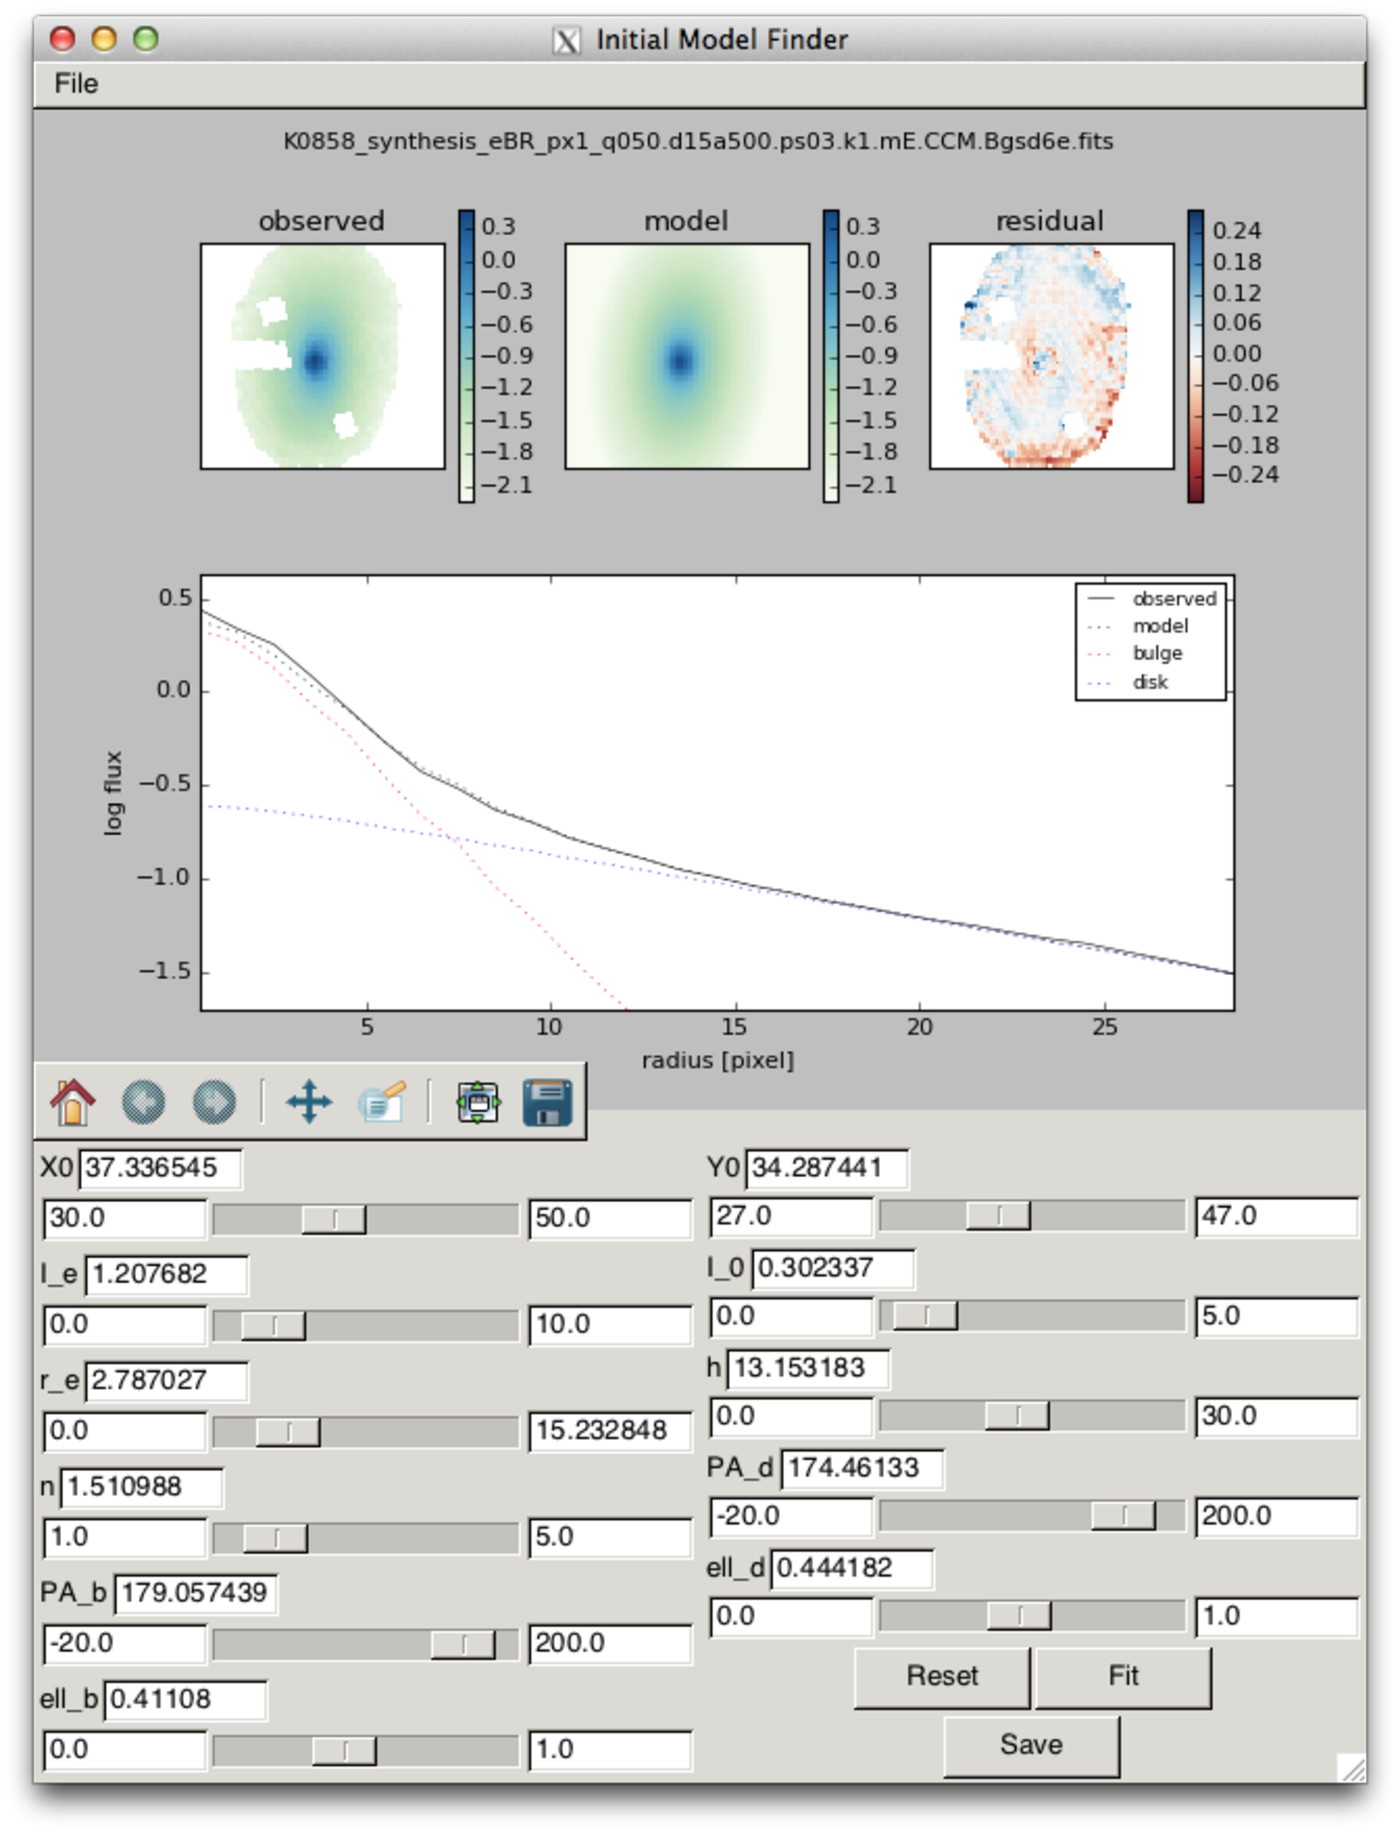
\includegraphics[width=1.0\columnwidth]{figuras/model_finder}
	\caption[Programa gráfico para encontrar o modelo inicial]
	{Programa gráfico para encontrar o modelo inicial de forma interativa.}
	\label{fig:modelFinder}
\end{figure}

Este procedimento é computacionalmente intensivo, e o conjunto de heurísticas
foi determinado de forma empírica. Ainda assim, ele falha em muitos casos,
geralmente precisando ser modificado caso a caso. O tempo típico, em um
computador atual, de ajuste do modelo inicial é de 10 minutos. É possível fazer
este ajuste de forma interativa, utilizando uma ferramenta gráfica, numa fração
deste tempo. Com este objetivo foi desenvolvido o programa mostrado na Figura
\ref{fig:modelFinder}. Com ele podem-se escolher modelos iniciais, limites, e
fazer um ajuste de teste, tudo em tempo real. Como a amostra é pequena, um
programa interativo ainda é uma abordagem viável.

Como visto na Seção \ref{sec:morph:comp:depLambda}, os parâmetros morfológicos
podem depender do comprimento de onda. Logo, um único modelo inicial pode não
ser suficiente para escapar dos mínimos locais. Assim, utiliza-se imagens em
caixas de $100\,\angstrom$, e espaçadas em intervalos também de
$100\,\angstrom$, para fazer ajustes utilizando o algoritmo N-M. Obtém-se desta
forma modelos iniciais para cada comprimento de onda. Os parâmetros destes
modelos são, de forma independente, ajustados a polinômios em função de
$\lambda$. Em nenhum caso (da amostra final deste trabalho) houve necessidade de
ajuste de um polinômio de ordem maior que 1, isto é, uma reta.

O ajuste morfológico final se dá utilizando os chutes iniciais dados pelos
polinômios dos parâmetros. As imagens são tomadas $\lambda$-a-$\lambda$, sem
combinar imagens. O ajuste é feito utilizando L-M. Caso não haja convergência do
algoritmo, ou o melhor ajuste fique preso em algum limite dos parâmetros, o
ajuste é marcado como falho.

Ao final do ajuste morfológico, cria-se uma imagem para o bojo e para o disco em
cada comprimento de onda. Os cubos de dados espectrais são montados apenas
armazenando estas imagens em ordem de comprimento de onda. Os cubos de dados
espectrais das componentes morfológicos estão prontos para serem analisados como
espectros.


%***************************************************************%
%                                                               %
%                      Seleção da amostra                       %
%                                                               %
%***************************************************************%

\section{Seleção da amostra de galáxias}

A amostra para candidatos à decomposição morfológica espectral foi selecionada a
partir de 331 galáxias observadas com a configuração V500, as quais passaram
pelo QBICK e tiveram os espectros passados pelo \starlight, sem segmentação em
zonas de Voronoi (ver Seções \ref{sec:ifs:qbick} e \ref{sec:ifs:starlight}).
Isto é necessário para que se tenham medidas da cinemática da galáxia,
utilizadas para preparar os dados antes da decomposição.

O passo seguinte foi selecionar as galáxias conforme seu tipo morfológico. A
classificação morfológica das galáxias da amostra mãe do CALIFA foi feita
visualmente por 5 voluntários, utilizando imagens do SDSS nas bandas $r$ e $i$
\citep{Walcher2014}. Os critérios foram:

\begin{itemize}
  \item Elíptica (E), com subclasse 0--7.
  \item Espiral (S), com subclasses 0, 0a, a, ab, b, bc, c, cd, d, m;
  \item Irregular (I);
  \item Em qualquer classe, barra (B), sem barra (A), ou indefinida (AB);
  \item Características de {\em merger} (sim ou não).
\end{itemize}

Os três primeiros itens formam uma sequência numérica segundo a classificação de
Hubble, de 0 a 18. As 5 classificações independentes foram combinadas,
calculando a média (descartando valores atípicos, distante mais de 4 classes da
média). Os valores máximos e mínimos, para dar uma ideia da incerteza, são
calculados utilizando todas as 5 classificações. Foi feita uma filtragem na
lista de galáxias observadas, baseada na tabela de classificação morfológica.
Dada a natureza subjetiva da classificação visual, optou-se por utilizar as
classificações máxima e mínima, de tal forma que seja possível que galáxia em
questão seja da classe S0. Isto é, se a galáxia for classificada como elíptica
($<\mathrm{S0}$), mas a classificação máxima for, por exemplo, Sa
($>\mathrm{S0}$), a galáxia entra na amostra. O inverso também vale, uma galáxia
Sa tiver uma classificação mínima E7, também entra na amostra.
As galáxias também têm que ser sem barra (A), e sem características de {\em
merger}.

Adicionalmente, as galáxias precisam ter uma elipticidade máxima $\epsilon<0,5$,
medida nas imagens do SDSS na banda $r$. Isto é necessário para evitar problemas
na decomposição morfológica, pois o modelo bojo--disco não funciona bem em
sistemas muito inclinados. A amostra inicial é listada na Tabela
\ref{tab:DecompSample} (Anexo \ref{apendice:amostra}).

O programa interativo de ajuste foi utilizado nas 43 galáxias da amostra.
O ajuste não pode ser feito em 19 delas, pois apresentaram características que
não permitem fazer a decomposição morfológica em bojo e disco, como faixas de
poeira ou disco muito fraco. Outras 15 apresentam problemas no ajuste, como
mínimos locais intermitentes ou ausência de alguma componente. A coluna de
observações na Tabela \ref{tab:DecompSample} informa os problemas encontrados em
cada caso. O sumário dos descartes é o seguinte:

\begin{itemize}
  \item Ajuste ruim: 15
  \item Faixa de poeira: 9
  \item Disco fraco: 5
  \item Inclinada: 2
  \item Braço espiral: 1
  \item Irregular: 1
  \item Poucos {\em spaxels}: 1
\end{itemize}

\begin{table}
\begin{tabular}{ l l r r r r l }
\hline
ID & Nome & Classe & Classe (mín.) & Classe (máx.) & $\epsilon$ \\
\hline
K0018 & NGC 0155  &  1 (E1)  & 0 (E0) &  8 (S0)  & $0,22$ \\
K0127 & NGC 1349  &  6 (E6)  & 0 (E0) & 10 (Sa)  & $0,11$ \\
K0592 & NGC 4874  &  0 (E0)  & 0 (E0) &  8 (S0)  & $0,12$ \\
K0602 & NGC 4956  &  1 (E1)  & 0 (E0) &  8 (S0)  & $0,14$ \\
K0832 & NGC 6146  &  5 (E5)  & 3 (E3) &  8 (S0)  & $0,23$ \\
K0846 & UGC 10695 &  5 (E5)  & 2 (E2) &  8 (S0)  & $0,33$ \\
K0851 & NGC 6338  &  5 (E5)  & 1 (E1) &  8 (S0)  & $0,34$ \\
K0858 & UGC 10905 &  9 (S0a) & 7 (E7) & 11 (Sab) & $0,47$ \\
K0912 & NGC 7623  &  8 (S0)  & 8 (S0) &  8 (S0)  & $0,29$ \\
\hline
\end{tabular}
\caption[Amostra final para decomposição morfológica espectral]
{Amostra final para decomposição morfológica espectral.}
\label{tab:DecompSampleFinal}
\end{table}

A identificação dos ajustes ditos ruins foi feita através de inspeção visual,
com um grau considerável de subjetividade. Os critérios incluem, por exemplo, a
presença de mínimos locais intermitentes e degenerados (parâmetros saltando
entre dois patamares com mudança imperceptível no aspecto dos perfis e no
$\chi^2$). Esta seleção foi feita de forma fortemente conservadora. A amostra
final deste trabalho (listada na Tabela \ref{tab:DecompSampleFinal}) consiste em
9 galáxias que tiveram uma decomposição boa segundo estes critérios.


%***************************************************************%
%                                                               %
%                  Decomposição da amostra final                %
%                                                               %
%***************************************************************%
\section{Aplicação da decomposição na amostra final}
\label{sec:Decomp:decomp}

A decomposição morfológica espectral foi realizada nas 9 galáxias da amostra
final. Figuras mostrando o resultado da decomposição de todas as galáxias podem
ser vistas no Apêndice \ref{apendice:Decomp}. Nesta seção é discutido o
resultado apenas para a galáxia em que se obteve a melhor decomposição, K0858
(UGC 10905). Recomenda-se comparar as figuras das outras galáxias com o que está
exposto a seguir.

\begin{figure}
	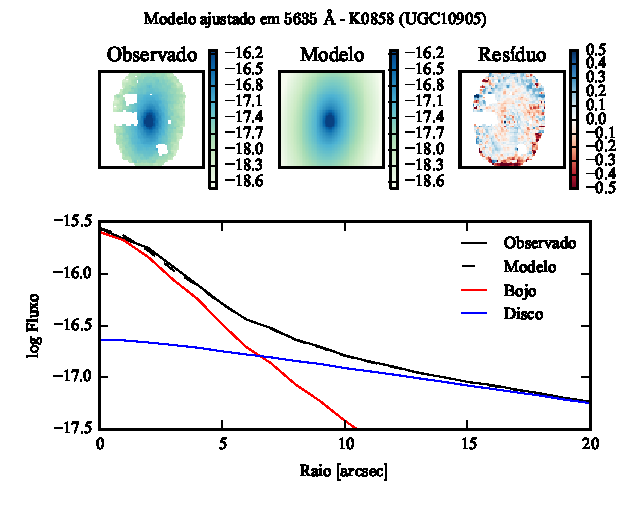
\includegraphics[page=1]{figuras-decomp/K0858_sample006a}
	\caption[Ajuste morfológico em $5635\,\angstrom$ para K0858 (UGC 10905)]
	{Acima: imagens observada, modelada e resíduo do fluxo em $5635\,\angstrom$
	para K0858 (UGC 10905). Abaixo: perfis radiais, obtidos pela média do fluxo em
	anéis elípticos nas imagens. O fluxo observado é representado pela linha preta
	sólida. O melhor ajuste é representado pela linha preta tracejada. O bojo e o
	disco que compõem o modelo são mostrados em vermelho e azul, respectivamente.}
	\label{fig:decompRadprof}
\end{figure}

A Figura \ref{fig:decompRadprof} permite uma visualização bidimensional, nos
painéis superiores, do fluxo observado, modelo e resíduo em $5635\,\angstrom$.
No resíduo se observam efeitos de borda próximos às regiões externas mascaradas,
além de artefatos seguindo um padrão quase regular\footnote{O padrão hexagonal
que aparece nas imagens (sobretudo nas de resíduo) está relacionado com a forma
como os cubos são reconstruídos.}. Pode-se observar também uma estrutura que
parece ser um braço espiral, em excesso (azul) no resíduo. Isto não é surpresa,
dado que esta galáxia é classificada como S0a. Outra forma de visualizar a
qualidade do ajuste é através do perfil de brilho radial, no painel inferior. O
perfil é calculado utilizando anéis elípticos, com a elipticidade calculada a
partir da imagem observada.

\begin{figure}
	\includegraphics[page=2]{figuras-decomp/K0858_sample006a}
	\caption[Parâmetros morfológicos em função do comprimento de onda para K0858
	(UGC 10905)]
	{Parâmetros morfológicos em função do comprimento de onda para
	K0858 (UGC 10905). Regiões em rosa representam comprimentos de onda onde a
	decomposição falhou. Regiões em cinza foram mascaradas antes de iniciar a
	decomposição. Pontos azuis indicam o primeiro passo da decomposição, em caixas
	de $100\,\angstrom$.}
	\label{fig:decompParams}
\end{figure}

A dependência em $\lambda$ dos parâmetros morfológicos obtidos para K0858 é
mostrada na Figura \ref{fig:decompParams}. As linhas pretas representam a
decomposição final, feita $\lambda$-a-$\lambda$, e os pontos azuis a
decomposição feita no primeiro passo da decomposição, em caixas de
$100\,\angstrom$. Regiões espectrais mascaradas antes de iniciar a decomposição
(onde pode haver emissão de gás) estão marcadas em cinza. Marcadas em rosa estão
regiões espectrais onde a decomposição falhou, quando o algoritmo não convergiu
ou ficou preso nos limites dos parâmetros.

A primeira coisa que chama a atenção na Figura \ref{fig:decompParams} é a
diferença entre as parâmetros morfológicos obtidos em caixas de $100\,\angstrom$
e os obtidos em a cada comprimento de onda. Isto pode ser devido à correção da
cinemática (Seção \ref{sec:Decomp:cinematica}), que praticamente não tem efeito
numa imagem de banda espectral larga. Pode também estar relacionado ao
sinal--ruído das imagens, que aumenta quando se soma imagens. De qualquer forma,
estamos interessados apenas no espectro; sendo assim, leva-se em conta apenas a
decomposição final.

Pode-se observar um gradiente espectral no comprimento de escala do disco ($h$).
Já o raio efetivo do bojo ($r_e$) e o índice de Sérsic ($n$) não apresentam um
gradiente apreciável. Todos os parâmetros parecem ter um salto em
$4000\,\angstrom$. O ajuste falha em comprimentos de onda menores, ficando
difícil determinar se isto é um resultado espúrio. Na verdade, qualquer
tentativa de interpretação, observando apenas a dependência dos parâmetros
morfológicos com o comprimento de onda, deve ser feita com cuidado. É esperado
que os parâmetros variem com o comprimento de onda, quando são medidos em bandas
espectrais largas e distantes, como mencionado na Seção
\ref{sec:morph:comp:depLambda}. Entretanto, estas são evidências empíricas, sem
um modelo que as suportem. Tirar conclusões da variação $\lambda$-a-$\lambda$
dos parâmetros pode ser precipitado.

\begin{figure}
	\includegraphics[page=4]{figuras-decomp/K0858_sample006a}
	\caption[Espectro das componentes morfológicas de K0858 (UGC 10905). Acima,
	espectros] {Espectro das componentes morfológicas de K0858 (UGC 10905),
	observado (preto), bojo (vermelho), disco (azul) e resíduo (magenta). Acima:
	Espectro do {\em spaxel} nuclear da galáxia. Meio: Espectro em um {\em spaxel}
	a uma distância de $r_e$ do núcleo. Abaixo: Espectro integrado espacialmente.}
	\label{fig:decompSpectra}
\end{figure}

Os espectros de galáxias, por outro lado, são melhor compreendidos. Mesmo as
menores características dos espectros, como linhas fracas de absorção, podem ser
razoavelmente bem explicadas com modelos de populações estelares. Então, se um
espectro de bojo ou disco tiver o aspecto de um espectro de galáxia, pode-se
começar a levar o resultado da decomposição a sério. A Figura
\ref{fig:decompSpectra} mostra os espectros dos modelos (bojo em vermelho e
disco em azul), no {\em spaxel} nuclear, a $r_e$ de distância do núcleo, e o
espectro integrado dos modelos. O espectro observado é mostrado em preto, e o
resíduo em magenta.

Com uma análise visual, os espectros parecem galáticos. Nos piores casos os
bojos parecem ter um ajuste pior do que os discos, e costumam ter dimensões
comparáveis à largura da PSF. A má resolução dos bojos pode comprometer a
decomposição, nestes casos. Pode-se observar que o resíduo geralmente apresenta
um gradiente nos {\em spaxels}, e praticamente desaparece no espectro integrado.
Este gradiente no resíduo indica que os modelos somados são mais vermelhos do
que o espectro observado. Isto certamente irá afetar o resultado da síntese de
populações estelares, analisada na seção a seguir. Os espectros integrados dos
modelos, se tiverem tal gradiente de cor, devem ter uma forma tal que se
cancelam no resíduo.

%***************************************************************%
%                                                               %
%                        Síntese espectral                      %
%                                                               %
%***************************************************************%
\section{Síntese espectral de populações estelares}
\label{sec:Decomp:sintese}

A síntese espectral de populações estelares utilizando \starlight foi aplicada
às componentes morfológicas e ao espectro original de todas as galáxias da
amostra final. A base utilizada foi a de Granada--MILES. Dentre as galáxias da
amostra, apenas duas tiveram um ajuste bom com o \starlight: K0592 e K0858. Os
espectros ajustados e as propriedades obtidas para toda a amostra estão no
Apêndice \ref{apendice:Decomp}. A seguir uma discussão sobre o resultado para
K0858.

\begin{figure}
	\includegraphics[page=15,width=\textwidth]{figuras/sample006a_synthesis}
	\caption[Espectros ajustados com \starlight das componentes morfológicas de
	K0858 (UGC 10905)]
	{Acima: Espectros integrados das componentes morfológicas de
	K0858 (UGC 10905), ajustados com \starlight. Em preto, espectro observado. Em
	vermelho, e azul, as componentes bojo e disco. Em linhas de cor clara, o
	espectro ajustado pelo \starlight. Abaixo: Resíduo dos espectros (observado
	menos sintético, divididos pelo observado).}
	\label{fig:decompSinteseSpec}
\end{figure}

A Figura \ref{fig:decompSinteseSpec} mostra ajustes do \starlight para os
espectros integrados observado, do bojo e do disco. As linhas mais claras
mostram o melhor ajuste. No painel inferior, tem-se o resíduo do ajuste em
relação ao espectro de entrada. O ajuste é bom em linhas gerais, embora seja
possível ver alguns pontos onde o resíduo do bojo e do disco estejam
anti-correlacionados, devido à degenerescência do modelo.


\begin{figure}
	\includegraphics[page=16]{figuras/sample006a_synthesis}
	\caption[Propriedades físicas das componentes morfológicas de K0858 (UGC 10905)]
	{Perfil radial de propriedades físicas das componentes morfológicas de
	K0858 (UGC 10905), obtidos através do \starlight. As linhas contínuas
	representam as propriedades obtidas utilizando espectros espacialmente
	resolvidos. As linhas tracejadas representam as propriedades obtidas utilizando
	os espectros integrados. Em preto, espectro observado. Em vermelho, e azul, as
	componentes bojo e disco. Acima, à esquerda: idade estelar média ponderada pela
	luminosidade. Acima, à direita: atenuação por poeira, na banda $V$. Abaixo, à
	esquerda: metalicidade estelar média, ponderada pela massa. Abaixo, à direita:
	densidade superficial de massa estelar. As frações de massa e luminosidade
	entre as componentes e a total (obtida do espectro observado) são indicadas no
	painel inferior, à direita.}
	\label{fig:decompSinteseRadprof}
\end{figure}

As propriedades físicas derivadas da síntese de populações estelares é mostrada
na Figura \ref{fig:decompSinteseRadprof}. Ali, pode-se ver um perfil radial das
propriedades, ajustados nos espectros de cada {\em spaxel}, ou seja,
espacialmente resolvidos, em linhas sólidas. As propriedades derivadas do
espectro integrado são mostradas como linhas tracejadas. Pode-se notar que a
atenuação por poeira $A_V$ (painel superior direito), tanto no bojo quanto no
disco, é muito diferente da atenuação para os espectros observados quando se
utilizam os espectros espacialmente resolvidos. O mesmo se observa para a idade
estelar média ponderada pela luminosidade (painel superior esquerdo). Estes dois
fatos provavelmente têm relação com o gradiente de cor aparente no resíduo da
decomposição morfológica espectral. A metalicidade estelar média ponderada pela
massa (painel inferior esquerdo), quando espacialmente resolvida, é muito
diferente da calculada no espectro integrado, para todos os casos. A densidade
superficial de massa estelar é mostrada no painel inferior direito. A massa e a
luminosidade das componentes morfológicas, em relação à massa da galáxia
original, são mostrados no mesmo painel. Note que, devido à quantidade de
poeira, a densidade de massa superficial espacialmente resolvida das componentes
morfológicas é maior do que a calculada com o espectro observado. Estes
problemas com a idade estelar e a atenuação por poeira, nos espectros
espacialmente resolvidos, aparecem também nas outras galáxias da amostra, mesmo
na outra galáxia com um bom ajuste de populações estelares, a K0592.

% TODO: inserir um parágrafo especulativo sobre poeira / idade, a pedido da
% Natalia.

\begin{figure}
	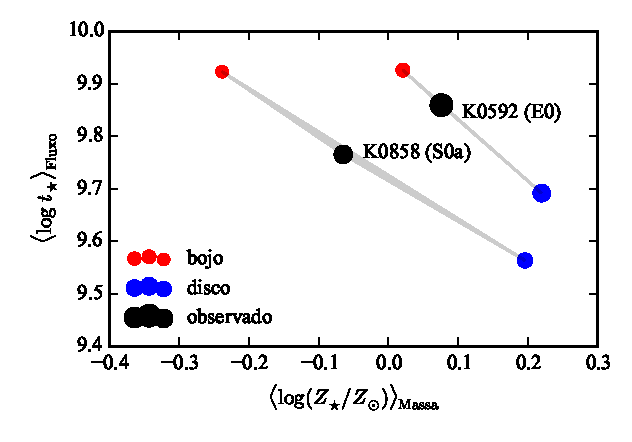
\includegraphics{figuras/sample006a_synthesis_all2}
	\caption[Idade e metalicidade médios das componentes morfológicas]
	{Idade estelar média ponderada pela luminosidade contra metalicidade estelar
	média ponderada pela massa, para as componentes duas morfológicas de
	duas galáxias do CALIFA: K0592 (NGC 4874, E0) e K0858 (UGC10905, S0a). Idades
	e metalicidades foram obtidas pelo \starlight. Pontos em preto são referentes
	ao espectro observado, total da galáxia. Pontos em vermelho são referentes
	ao bojo, e em azul, ao disco. A área dos círculos indica a massa estelar.}
	\label{fig:decompSintese}
\end{figure}

As propriedades obtidas com os espectros integrados, por outro lado, parecem
melhor comportadas. A Figura \ref{fig:decompSintese} mostra um gráfico da idade
contra metalicidade estelar, para as componentes morfológicas (bojo em vermelho
e disco em azul) e para o espectro observado (em preto) de K0592 e K0858. A
massa da galáxia (ou da componente morfológica) é representada pela área do
círculo.
As duas galáxias, neste gráfico, têm um comportamento similar.
Ambas têm um bojo mais velho e de metalicidade mais baixa, e um disco mais jovem
e de metalicidade mais alta, com relação à idade e metalicidade do espectro
observado. Também é interessante notar que os pontos para uma mesma galáxia
estão alinhados. Isto pode acontecer devido à degenerescência entre idade e
metalicidade, comumente vista em sínteses de população estelar.

\begin{figure}
	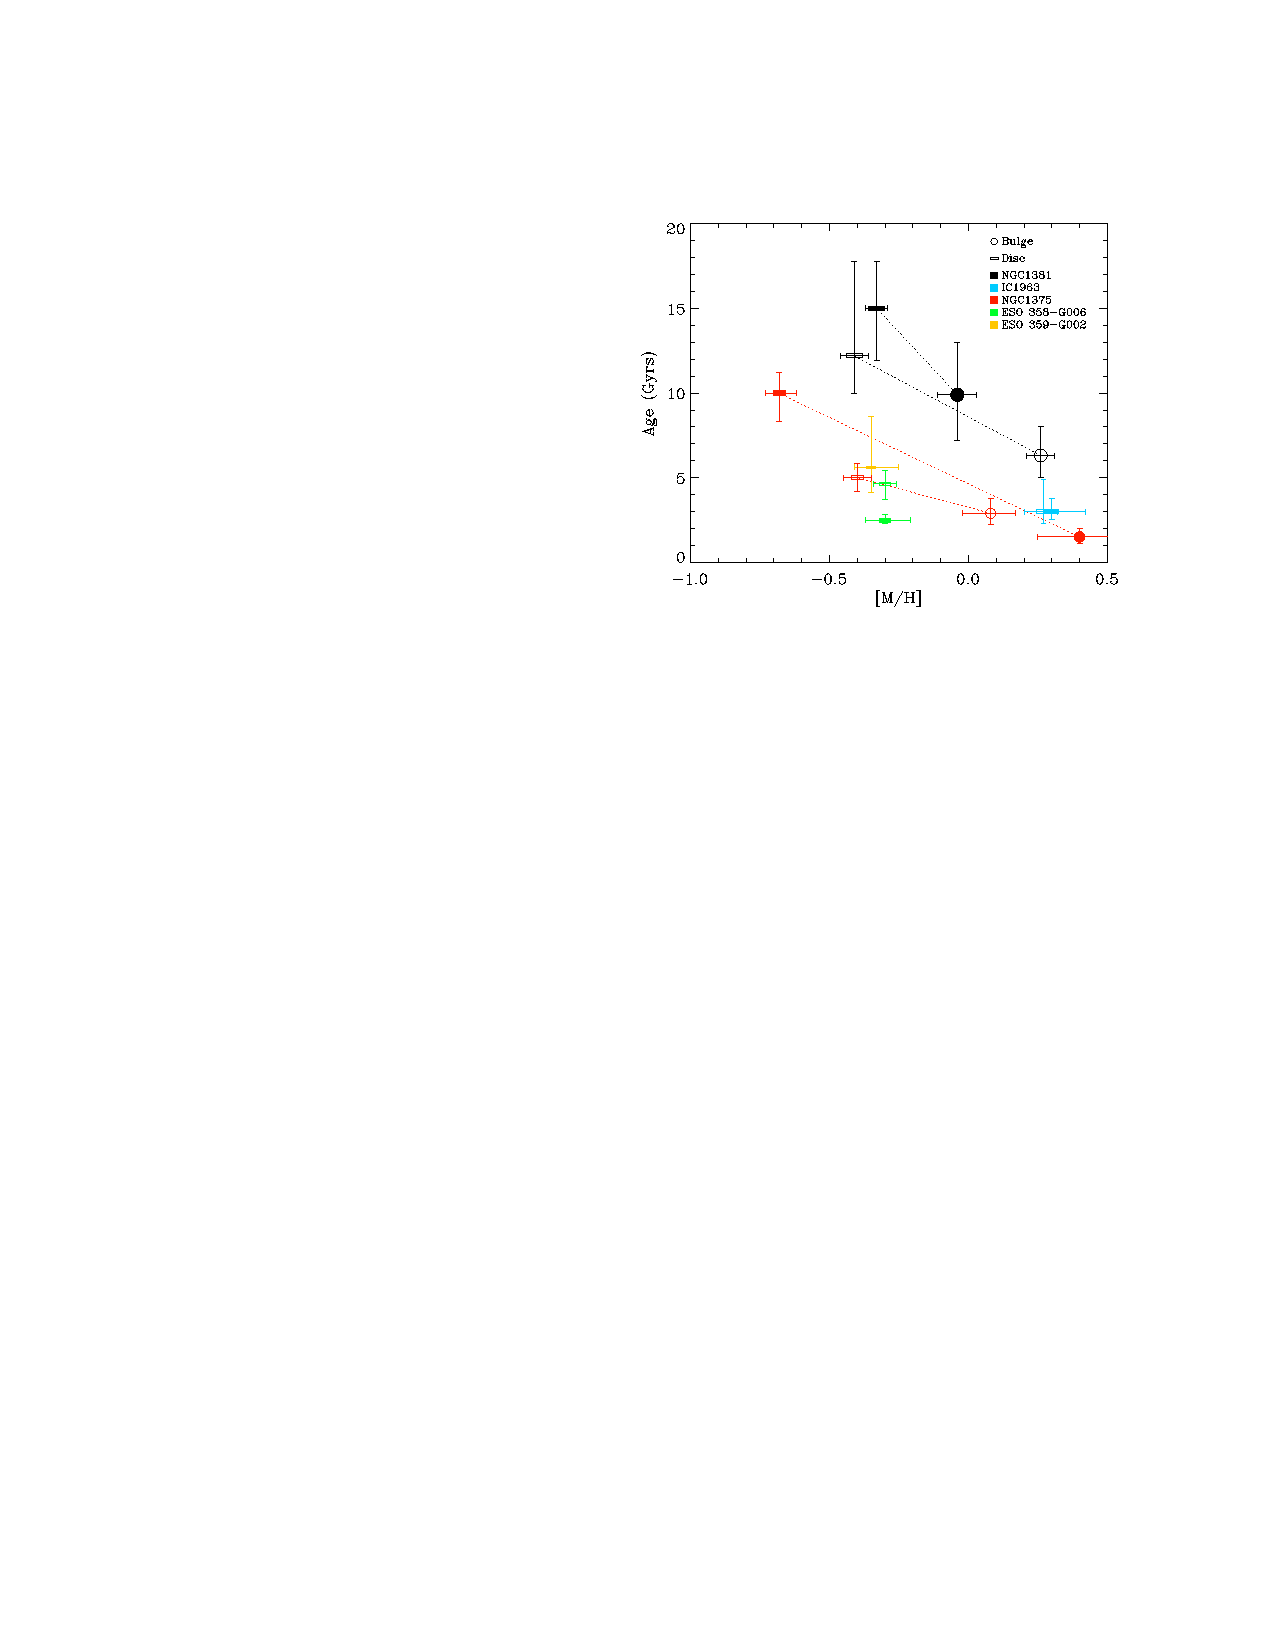
\includegraphics[width=0.9\textwidth]{figuras/johnston-pop}
	\caption[A mesma Figura que \ref{fig:populationJohnston}] {A mesma Figura que
	\ref{fig:populationJohnston}, mostrada novamente para comparar com a Figura
	\ref{fig:decompSintese}.}
	\label{fig:populationJohnston2}
\end{figure}

É interessante comparar a Figura \ref{fig:decompSintese} com o resultado de
\citet{Johnston2012}, reproduzido na Figura \ref{fig:populationJohnston2}.
Os resultados obtidos aqui, embora não tenham significância estatística, são
contrários ao resultado de \citeauthor{Johnston2012}, que obtêm, para galáxias
S0, bojos mais jovens e mais metálicos que seus discos. Tanto a idade quanto a
metalicidade que eles utilizam foram obtidos através do ajuste de duas linhas de
absorção, enquanto neste trabalho o espectro inteiro foi utilizado no ajuste de
populações estelares.

Além disso, eles trabalham com perfis unidimensionais (espectros de fenda
longa), enquanto análise feita aqui é toda em 2-D (imagens). Por fim, não é
óbvio que as galáxias de nossa amostra sejam comparáveis à da amostra de
\citeauthor{Johnston2012}. De fato, apesar de ambas amostras selecionarem
galáxias S0, as galáxias de \citeauthor{Johnston2012} parecem ser menos massivas
que as nossas. Enquanto K0858 tem magnitude absoluta na banda $B$ de $M_B = -21$
(K0592 tem medida somente na banda $V$, com $M_V = -23,6$), as de
\citeauthor{Johnston2012} $M_B$ entre $-17$ e $-19$.

Todas essas diferenças complicam a comparação dos resultados obtidos neste
trabalho com aqueles do artigo que inspirou todo esse estudo. De qualquer modo,
os experimentos aqui reportados mostram que a decomposição morfológica espectral
é um problema bastante mais delicado do que se imaginava anteriormente.


%% End of this chapter
